\documentclass[10pt,twoside,openany]{memoir}
\usepackage[T1]{fontenc}
%\usepackage{tgpagella} % text only
%\usepackage{mathpazo}  % math & text
\usepackage[T1]{fontenc}
\usepackage[margin=1.5in]{geometry}
\usepackage[hidelinks]{hyperref}
\usepackage{amsmath}
\usepackage{amsthm}
\usepackage{amssymb}
\usepackage{mathtools}
\usepackage{graphicx}
%\usepackage{newpxtext}
%\usepackage{eulerpx}
%\usepackage{eucal}
\usepackage{datetime}
    \newdateformat{specialdate}{\THEYEAR\ \monthname\ \THEDAY}
\usepackage{fancyhdr}
    \fancyhf{}
    \pagestyle{fancy}
    \cfoot{\scriptsize \thepage}
    \fancyhead[R]{\scriptsize \rightmark}
    \fancyhead[L]{\scriptsize \leftmark}
    \renewcommand{\headrulewidth}{0pt}
    \renewcommand{\footrulewidth}{0pt} % if you also want to remove the footer rule
\usepackage{mdframed}
\usepackage{pdfpages}
\mdfsetup{font=\small}

\mdfdefinestyle{mystyle}{linecolor=black }


\usepackage{thmtools}
    \declaretheoremstyle[
        spaceabove=10pt,
        spacebelow=10pt,
        headfont=\normalfont\bfseries,
        notefont=\mdseries, notebraces={(}{)},
        bodyfont=\normalfont,
        postheadspace=0.5em
        %qed=\qedsymbol
        ]{defs}

    \declaretheoremstyle[ 
        spaceabove=10pt, % space above the theorem
        spacebelow=10pt,
        headfont=\normalfont\bfseries,
        bodyfont=\normalfont\itshape,
        postheadspace=0.5em
        ]{thmstyle}
    
    \declaretheorem[
        style=thmstyle,
        numberwithin=section
    ]{theorem}

    \declaretheorem[
        style=thmstyle,
        sibling=theorem,
    ]{proposition}

    \declaretheorem[
        style=thmstyle,
        sibling=theorem,
    ]{lemma}

    \declaretheorem[
        style=thmstyle,
        sibling=theorem,
    ]{corollary}

    \declaretheorem[
        numberwithin=section,
        style=defs,
    ]{example}

    \declaretheorem[
        numberwithin=section,
        style=defs,
    ]{definition}

    \declaretheorem[
        style=defs,
        numbered=unless unique,
    ]{problem}

    \declaretheorem[
        numbered=unless unique,
        shaded={rulecolor=black,
    rulewidth=1pt, bgcolor={rgb}{1,1,1}}
    ]{axiom}

    \declaretheorem[numberwithin=section,style=defs]{note}
    \declaretheorem[style=defs]{exercise}
    \declaretheorem[numbered=no,style=defs]{question}
    \declaretheorem[numbered=no,style=defs]{recall}
    \declaretheorem[numbered=no,style=remark]{answer}
    \declaretheorem[numbered=no,style=remark]{solution}

    \declaretheorem[numbered=no,style=defs]{remark}
\usepackage{enumitem}
\usepackage{titlesec}
    \titleformat{\chapter}[display]
    {\bfseries\LARGE\raggedright}
    {Chapter {\thechapter}}
    {1ex minus .1ex}
    {\Huge}
    \titlespacing{\chapter}
    {3pc}{*3}{40pt}[3pc]

    \titleformat{\section}[block]
    {\normalfont\bfseries\Large}
    {\S\ \thesection.}{.5em}{}[]
    \titlespacing{\section}
    {0pt}{3ex plus .1ex minus .2ex}{3ex plus .1ex minus .2ex}
\usepackage[utf8x]{inputenc}
\usepackage{tikz}
\usepackage{tikz-cd}
\usepackage{wasysym}
\usepackage{pgf}
\usepackage{mmacells}
\usepackage{listings}
\usepackage{xcolor}

\definecolor{codegreen}{rgb}{0,0.6,0}
\definecolor{codegray}{rgb}{0.5,0.5,0.5}
\definecolor{codepurple}{rgb}{0.58,0,0.82}
\definecolor{backcolour}{rgb}{0.95,0.95,0.92}

\lstdefinestyle{mystyle}{
    backgroundcolor=\color{backcolour},   
    commentstyle=\color{codegreen},
    keywordstyle=\color{magenta},
    numberstyle=\tiny\color{codegray},
    stringstyle=\color{codepurple},
    basicstyle=\ttfamily\footnotesize,
    breakatwhitespace=false,         
    breaklines=true,                 
    captionpos=b,                    
    keepspaces=true,                 
    numbers=left,                    
    numbersep=5pt,                  
    showspaces=false,                
    showstringspaces=false,
    showtabs=false,                  
    tabsize=2
}

\lstset{style=mystyle}
\usepackage{fancyvrb}
\usepackage{tcolorbox}

% Define replacements: "what to look for" => "how to typeset it"
\mmaDefineMathReplacement[≤]{<=}{\leq}
\mmaDefineMathReplacement[≥]{>=}{\geq}
\mmaDefineMathReplacement[≠]{!=}{\neq}
\mmaDefineMathReplacement[→]{->}{\to}[2]
\mmaDefineMathReplacement[⧴]{:>}{:\hspace{-.2em}\to}[2]
\mmaDefineMathReplacement{∉}{\notin}
\mmaDefineMathReplacement{∞}{\infty}
\mmaDefineMathReplacement{𝕕}{\mathbbm{d}}

\linespread{1}
%to make the correct symbol for Sha
%\newcommand\cyr{%
%\renewcommand\rmdefault{wncyr}%
%\renewcommand\sfdefault{wncyss}%
%\renewcommand\encodingdefault{OT2}%
%\normalfont \selectfont} \DeclareTextFontCommand{\textcyr}{\cyr}


\DeclareMathOperator{\ab}{ab}
\newcommand{\absgal}{\G_{\bbQ}}
\DeclareMathOperator{\ad}{ad}
\DeclareMathOperator{\adj}{adj}
\DeclareMathOperator{\alg}{alg}
\DeclareMathOperator{\Alt}{Alt}
\DeclareMathOperator{\Ann}{Ann}
\DeclareMathOperator{\arith}{arith}
\DeclareMathOperator{\Aut}{Aut}
\DeclareMathOperator{\Be}{B}
\DeclareMathOperator{\Bd}{Bd}
\DeclareMathOperator{\card}{card}
\DeclareMathOperator{\Char}{char}
\DeclareMathOperator{\csp}{csp}
\DeclareMathOperator{\codim}{codim}
\DeclareMathOperator{\coker}{coker}
\DeclareMathOperator{\coh}{H}
\DeclareMathOperator{\compl}{compl}
\DeclareMathOperator{\conj}{conj}
\DeclareMathOperator{\cont}{cont}
\DeclareMathOperator{\Cov}{Cov}
\DeclareMathOperator{\crys}{crys}
\DeclareMathOperator{\Crys}{Crys}
\DeclareMathOperator{\cusp}{cusp}
\DeclareMathOperator{\diag}{diag}
\DeclareMathOperator{\diam}{diam}
\DeclareMathOperator{\Dom}{Dom}
\DeclareMathOperator{\disc}{disc}
\DeclareMathOperator{\dist}{dist}
\DeclareMathOperator{\dR}{dR}
\DeclareMathOperator{\Eis}{Eis}
\DeclareMathOperator{\End}{End}
\DeclareMathOperator{\ev}{ev}
\DeclareMathOperator{\eval}{eval}
\DeclareMathOperator{\Eq}{Eq}
\DeclareMathOperator{\Ext}{Ext}
\DeclareMathOperator{\Fil}{Fil}
\DeclareMathOperator{\Fitt}{Fitt}
\DeclareMathOperator{\Frob}{Frob}
\DeclareMathOperator{\G}{G}
\DeclareMathOperator{\Gal}{Gal}
\DeclareMathOperator{\GL}{GL}
\DeclareMathOperator{\Gr}{Gr}
\DeclareMathOperator{\Graph}{Graph}
\DeclareMathOperator{\GSp}{GSp}
\DeclareMathOperator{\GUn}{GU}
\DeclareMathOperator{\Hom}{Hom}
\DeclareMathOperator{\id}{id}
\DeclareMathOperator{\Id}{Id}
\DeclareMathOperator{\Ik}{Ik}
\DeclareMathOperator{\IM}{Im}
\DeclareMathOperator{\Image}{im}
\DeclareMathOperator{\Ind}{Ind}
\DeclareMathOperator{\Inf}{inf}
\DeclareMathOperator{\Isom}{Isom}
\DeclareMathOperator{\J}{J}
\DeclareMathOperator{\Jac}{Jac}
\DeclareMathOperator{\lcm}{lcm}
\DeclareMathOperator{\length}{length}
\DeclareMathOperator*{\limit}{limit}
\DeclareMathOperator{\Log}{Log}
\DeclareMathOperator{\M}{M}
\DeclareMathOperator{\Mat}{Mat}
\DeclareMathOperator{\N}{N}
\DeclareMathOperator{\Nm}{Nm}
\DeclareMathOperator{\NIk}{N-Ik}
\DeclareMathOperator{\NSK}{N-SK}
\DeclareMathOperator{\new}{new}
\DeclareMathOperator{\obj}{obj}
\DeclareMathOperator{\old}{old}
\DeclareMathOperator{\ord}{ord}
\DeclareMathOperator{\Or}{O}
\DeclareMathOperator{\op}{op}
\DeclareMathOperator{\PGL}{PGL}
\DeclareMathOperator{\PGSp}{PGSp}
\DeclareMathOperator{\rank}{rank}
\DeclareMathOperator{\Ran}{Ran}
\DeclareMathOperator{\Rel}{Rel}
\DeclareMathOperator{\Real}{Re}
\DeclareMathOperator{\RES}{res}
\DeclareMathOperator{\Res}{Res}
%\DeclareMathOperator{\Sha}{\textcyr{Sh}}
\DeclareMathOperator{\Sel}{Sel}
\DeclareMathOperator{\semi}{ss}
\DeclareMathOperator{\sgn}{sign}
\DeclareMathOperator{\SK}{SK}
\DeclareMathOperator{\SL}{SL}
\DeclareMathOperator{\SO}{SO}
\DeclareMathOperator{\Sp}{Sp}
\DeclareMathOperator{\Span}{span}
\DeclareMathOperator{\Spec}{Spec}
\DeclareMathOperator{\spin}{spin}
\DeclareMathOperator{\st}{st}
\DeclareMathOperator{\St}{St}
\DeclareMathOperator{\SUn}{SU}
\DeclareMathOperator{\supp}{supp}
\DeclareMathOperator{\Sup}{sup}
\DeclareMathOperator{\Sym}{Sym}
\DeclareMathOperator{\Tam}{Tam}
\DeclareMathOperator{\tors}{tors}
\DeclareMathOperator{\tr}{tr}
\DeclareMathOperator{\Tr}{Tr}
\DeclareMathOperator{\un}{un}
\DeclareMathOperator{\Un}{U}
\DeclareMathOperator{\val}{val}
\DeclareMathOperator{\vol}{vol}

\DeclareMathOperator{\Sets}{S \mkern1.04mu e \mkern1.04mu t \mkern1.04mu s}
    \newcommand{\cSets}{\scalebox{1.02}{\contour{black}{$\Sets$}}}
    
\DeclareMathOperator{\Groups}{G \mkern1.04mu r \mkern1.04mu o \mkern1.04mu u \mkern1.04mu p \mkern1.04mu s}
    \newcommand{\cGroups}{\scalebox{1.02}{\contour{black}{$\Groups$}}}

\DeclareMathOperator{\TTop}{T \mkern1.04mu o \mkern1.04mu p}
    \newcommand{\cTop}{\scalebox{1.02}{\contour{black}{$\TTop$}}}

\DeclareMathOperator{\Htp}{H \mkern1.04mu t \mkern1.04mu p}
    \newcommand{\cHtp}{\scalebox{1.02}{\contour{black}{$\Htp$}}}

\DeclareMathOperator{\Mod}{M \mkern1.04mu o \mkern1.04mu d}
    \newcommand{\cMod}{\scalebox{1.02}{\contour{black}{$\Mod$}}}

\DeclareMathOperator{\Ab}{A \mkern1.04mu b}
    \newcommand{\cAb}{\scalebox{1.02}{\contour{black}{$\Ab$}}}

\DeclareMathOperator{\Rings}{R \mkern1.04mu i \mkern1.04mu n \mkern1.04mu g \mkern1.04mu s}
    \newcommand{\cRings}{\scalebox{1.02}{\contour{black}{$\Rings$}}}

\DeclareMathOperator{\ComRings}{C \mkern1.04mu o \mkern1.04mu m \mkern1.04mu R \mkern1.04mu i \mkern1.04mu n \mkern1.04mu g \mkern1.04mu s}
    \newcommand{\cComRings}{\scalebox{1.05}{\contour{black}{$\ComRings$}}}

\DeclareMathOperator{\hHom}{H \mkern1.04mu o \mkern1.04mu m}
    \newcommand{\cHom}{\scalebox{1.02}{\contour{black}{$\hHom$}}}

\renewcommand{\k}{\kappa}
\newcommand{\Ff}{F_{f}}
%\newcommand{\ts}{\,^{t}\!}


%Mathcal
\newcommand{\cA}{\mathcal{A}}
\newcommand{\cB}{\mathcal{B}}
\newcommand{\cC}{\mathcal{C}}
\newcommand{\cD}{\mathcal{D}}
\newcommand{\cE}{\mathcal{E}}
\newcommand{\cF}{\mathcal{F}}
\newcommand{\cG}{\mathcal{G}}
\newcommand{\cH}{\mathcal{H}}
\newcommand{\cI}{\mathcal{I}}
\newcommand{\cJ}{\mathcal{J}}
\newcommand{\cK}{\mathcal{K}}
\newcommand{\cL}{\mathcal{L}}
\newcommand{\cM}{\mathcal{M}}
\newcommand{\cN}{\mathcal{N}}
\newcommand{\cO}{\mathcal{O}}
\newcommand{\cP}{\mathcal{P}}
\newcommand{\cQ}{\mathcal{Q}}
\newcommand{\cR}{\mathcal{R}}
\newcommand{\cS}{\mathcal{S}}
\newcommand{\cT}{\mathcal{T}}
\newcommand{\cU}{\mathcal{U}}
\newcommand{\cV}{\mathcal{V}}
\newcommand{\cW}{\mathcal{W}}
\newcommand{\cX}{\mathcal{X}}
\newcommand{\cY}{\mathcal{Y}}
\newcommand{\cZ}{\mathcal{Z}}


%mathfrak (missing \fi)
\newcommand{\fa}{\mathfrak{a}}
\newcommand{\fA}{\mathfrak{A}}
\newcommand{\fb}{\mathfrak{b}}
\newcommand{\fB}{\mathfrak{B}}
\newcommand{\fc}{\mathfrak{c}}
\newcommand{\fC}{\mathfrak{C}}
\newcommand{\fd}{\mathfrak{d}}
\newcommand{\fD}{\mathfrak{D}}
\newcommand{\fe}{\mathfrak{e}}
\newcommand{\fE}{\mathfrak{E}}
\newcommand{\ff}{\mathfrak{f}}
\newcommand{\fF}{\mathfrak{F}}
\newcommand{\fg}{\mathfrak{g}}
\newcommand{\fG}{\mathfrak{G}}
\newcommand{\fh}{\mathfrak{h}}
\newcommand{\fH}{\mathfrak{H}}
\newcommand{\fI}{\mathfrak{I}}
\newcommand{\fj}{\mathfrak{j}}
\newcommand{\fJ}{\mathfrak{J}}
\newcommand{\fk}{\mathfrak{k}}
\newcommand{\fK}{\mathfrak{K}}
\newcommand{\fl}{\mathfrak{l}}
\newcommand{\fL}{\mathfrak{L}}
\newcommand{\fm}{\mathfrak{m}}
\newcommand{\fM}{\mathfrak{M}}
\newcommand{\fn}{\mathfrak{n}}
\newcommand{\fN}{\mathfrak{N}}
\newcommand{\fo}{\mathfrak{o}}
\newcommand{\fO}{\mathfrak{O}}
\newcommand{\fp}{\mathfrak{p}}
\newcommand{\fP}{\mathfrak{P}}
\newcommand{\fq}{\mathfrak{q}}
\newcommand{\fQ}{\mathfrak{Q}}
\newcommand{\fr}{\mathfrak{r}}
\newcommand{\fR}{\mathfrak{R}}
\newcommand{\fs}{\mathfrak{s}}
\newcommand{\fS}{\mathfrak{S}}
\newcommand{\ft}{\mathfrak{t}}
\newcommand{\fT}{\mathfrak{T}}
\newcommand{\fu}{\mathfrak{u}}
\newcommand{\fU}{\mathfrak{U}}
\newcommand{\fv}{\mathfrak{v}}
\newcommand{\fV}{\mathfrak{V}}
\newcommand{\fw}{\mathfrak{w}}
\newcommand{\fW}{\mathfrak{W}}
\newcommand{\fx}{\mathfrak{x}}
\newcommand{\fX}{\mathfrak{X}}
\newcommand{\fy}{\mathfrak{y}}
\newcommand{\fY}{\mathfrak{Y}}
\newcommand{\fz}{\mathfrak{z}}
\newcommand{\fZ}{\mathfrak{Z}}


%mathbf
\newcommand{\bfA}{\mathbf{A}}
\newcommand{\bfB}{\mathbf{B}}
\newcommand{\bfC}{\mathbf{C}}
\newcommand{\bfD}{\mathbf{D}}
\newcommand{\bfE}{\mathbf{E}}
\newcommand{\bfF}{\mathbf{F}}
\newcommand{\bfG}{\mathbf{G}}
\newcommand{\bfH}{\mathbf{H}}
\newcommand{\bfI}{\mathbf{I}}
\newcommand{\bfJ}{\mathbf{J}}
\newcommand{\bfK}{\mathbf{K}}
\newcommand{\bfL}{\mathbf{L}}
\newcommand{\bfM}{\mathbf{M}}
\newcommand{\bfN}{\mathbf{N}}
\newcommand{\bfO}{\mathbf{O}}
\newcommand{\bfP}{\mathbf{P}}
\newcommand{\bfQ}{\mathbf{Q}}
\newcommand{\bfR}{\mathbf{R}}
\newcommand{\bfS}{\mathbf{S}}
\newcommand{\bfT}{\mathbf{T}}
\newcommand{\bfU}{\mathbf{U}}
\newcommand{\bfV}{\mathbf{V}}
\newcommand{\bfW}{\mathbf{W}}
\newcommand{\bfX}{\mathbf{X}}
\newcommand{\bfY}{\mathbf{Y}}
\newcommand{\bfZ}{\mathbf{Z}}

\newcommand{\bfa}{\mathbf{a}}
\newcommand{\bfb}{\mathbf{b}}
\newcommand{\bfc}{\mathbf{c}}
\newcommand{\bfd}{\mathbf{d}}
\newcommand{\bfe}{\mathbf{e}}
\newcommand{\bff}{\mathbf{f}}
\newcommand{\bfg}{\mathbf{g}}
\newcommand{\bfh}{\mathbf{h}}
\newcommand{\bfi}{\mathbf{i}}
\newcommand{\bfj}{\mathbf{j}}
\newcommand{\bfk}{\mathbf{k}}
\newcommand{\bfl}{\mathbf{l}}
\newcommand{\bfm}{\mathbf{m}}
\newcommand{\bfn}{\mathbf{n}}
\newcommand{\bfo}{\mathbf{o}}
\newcommand{\bfp}{\mathbf{p}}
\newcommand{\bfq}{\mathbf{q}}
\newcommand{\bfr}{\mathbf{r}}
\newcommand{\bfs}{\mathbf{s}}
\newcommand{\bft}{\mathbf{t}}
\newcommand{\bfu}{\mathbf{u}}
\newcommand{\bfv}{\mathbf{v}}
\newcommand{\bfw}{\mathbf{w}}
\newcommand{\bfx}{\mathbf{x}}
\newcommand{\bfy}{\mathbf{y}}
\newcommand{\bfz}{\mathbf{z}}

%blackboard bold

\newcommand{\bbA}{\mathbb{A}}
\newcommand{\bbB}{\mathbb{B}}
\newcommand{\bbC}{\mathbb{C}}
\newcommand{\bbD}{\mathbb{D}}
\newcommand{\bbE}{\mathbb{E}}
\newcommand{\bbF}{\mathbb{F}}
\newcommand{\bbG}{\mathbb{G}}
\newcommand{\bbH}{\mathbb{H}}
\newcommand{\bbI}{\mathbb{I}}
\newcommand{\bbJ}{\mathbb{J}}
\newcommand{\bbK}{\mathbb{K}}
\newcommand{\bbL}{\mathbb{L}}
\newcommand{\bbM}{\mathbb{M}}
\newcommand{\bbN}{\mathbb{N}}
\newcommand{\bbO}{\mathbb{O}}
\newcommand{\bbP}{\mathbb{P}}
\newcommand{\bbQ}{\mathbb{Q}}
\newcommand{\bbR}{\mathbb{R}}
\newcommand{\bbS}{\mathbb{S}}
\newcommand{\bbT}{\mathbb{T}}
\newcommand{\bbU}{\mathbb{U}}
\newcommand{\bbV}{\mathbb{V}}
\newcommand{\bbW}{\mathbb{W}}
\newcommand{\bbX}{\mathbb{X}}
\newcommand{\bbY}{\mathbb{Y}}
\newcommand{\bbZ}{\mathbb{Z}}
\newcommand{\jota}{\jmath}

\newcommand{\bmat}{\left( \begin{matrix}}
\newcommand{\emat}{\end{matrix} \right)}

\newcommand{\bbmat}{\left[ \begin{matrix}}
\newcommand{\ebmat}{\end{matrix} \right]}

\newcommand{\pmat}{\left( \begin{smallmatrix}}
\newcommand{\epmat}{\end{smallmatrix} \right)}

\newcommand{\lat}{\mathscr{L}}
\newcommand{\mat}[4]{\begin{pmatrix}{#1}&{#2}\\{#3}&{#4}\end{pmatrix}}
\newcommand{\ov}[1]{\overline{#1}}
\newcommand{\res}[1]{\underset{#1}{\RES}\,}
\newcommand{\up}{\upsilon}

\newcommand{\tac}{\textasteriskcentered}

%mahesh macros
\newcommand{\tm}{\textrm}

%Comments
\newcommand{\com}[1]{\vspace{5 mm}\par \noindent
\marginpar{\textsc{Comment}} \framebox{\begin{minipage}[c]{0.95
\textwidth} \tt #1 \end{minipage}}\vspace{5 mm}\par}

\newcommand{\Bmu}{\mbox{$\raisebox{-0.59ex}
  {$l$}\hspace{-0.18em}\mu\hspace{-0.88em}\raisebox{-0.98ex}{\scalebox{2}
  {$\color{white}.$}}\hspace{-0.416em}\raisebox{+0.88ex}
  {$\color{white}.$}\hspace{0.46em}$}{}}  %need graphicx and xcolor. this produces blackboard bold mu 

\newcommand{\hooktwoheadrightarrow}{%
  \hookrightarrow\mathrel{\mspace{-15mu}}\rightarrow
}

\makeatletter
\newcommand{\xhooktwoheadrightarrow}[2][]{%
  \lhook\joinrel
  \ext@arrow 0359\rightarrowfill@ {#1}{#2}%
  \mathrel{\mspace{-15mu}}\rightarrow
}
\makeatother

\renewcommand{\geq}{\geqslant}
\renewcommand{\leq}{\leqslant}
\newcommand{\midd}{\hspace{4pt}\middle|\hspace{4pt}}
    
\newcommand{\bone}{\mathbf{1}}
\newcommand{\sign}{\mathrm{sign}}
\newcommand{\eps}{\varepsilon}
\newcommand{\textui}[1]{\uline{\textit{#1}}}

%\newcommand{\ov}{\overline}
%\newcommand{\un}{\underline}
\newcommand{\fin}{\mathrm{fin}}

\newcommand{\chnum}{\titleformat
{\chapter} % command
[display] % shape
{\centering} % format
{\Huge \color{black} \shadowbox{\thechapter}} % label
{-0.5em} % sep (space between the number and title)
{\LARGE \color{black} \underline} % before-code
}

\newcommand{\chunnum}{\titleformat
{\chapter} % command
[display] % shape
{} % format
{} % label
{0em} % sep
{ \begin{flushright} \begin{tabular}{r}  \Huge \color{black}
} % before-code
[
\end{tabular} \end{flushright} \normalsize
] % after-code
}

\newcommand{\nl}{\newline \mbox{}}

\newcommand{\h}[1]{\hspace{#1pt}}

\newcommand{\littletaller}{\mathchoice{\vphantom{\big|}}{}{}{}}
\newcommand\restr[2]{{% we make the whole thing an ordinary symbol
  \left.\kern-\nulldelimiterspace % automatically resize the bar with \right
  #1 % the function
  \littletaller % pretend it's a little taller at normal size
  \right|_{#2} % this is the delimiter
  }}

\newcommand{\mtext}[1]{\hspace{6pt}\text{#1}\hspace{6pt}}

\newcommand{\lnorm}{\left\lVert}
\newcommand{\rnorm}{\right\rVert}

\newcommand{\ds}{\displaystyle}
\newcommand{\ts}{\textstyle}


\newcommand{\sfrac}[2]{{}^{#1}\mskip -5mu/\mskip -3mu_{#2}}


\makeatletter
\newcommand*{\da@rightarrow}{\mathchar"0\hexnumber@\symAMSa 4B }
\newcommand*{\da@leftarrow}{\mathchar"0\hexnumber@\symAMSa 4C }
\newcommand*{\xdashrightarrow}[2][]{%
  \mathrel{%
    \mathpalette{\da@xarrow{#1}{#2}{}\da@rightarrow{\,}{}}{}%
  }%
}
\newcommand{\xdashleftarrow}[2][]{%
  \mathrel{%
    \mathpalette{\da@xarrow{#1}{#2}\da@leftarrow{}{}{\,}}{}%
  }%
}
\newcommand*{\da@xarrow}[7]{%
  % #1: below
  % #2: above
  % #3: arrow left
  % #4: arrow right
  % #5: space left 
  % #6: space right
  % #7: math style 
  \sbox0{$\ifx#7\scriptstyle\scriptscriptstyle\else\scriptstyle\fi#5#1#6\m@th$}%
  \sbox2{$\ifx#7\scriptstyle\scriptscriptstyle\else\scriptstyle\fi#5#2#6\m@th$}%
  \sbox4{$#7\dabar@\m@th$}%
  \dimen@=\wd0 %
  \ifdim\wd2 >\dimen@
    \dimen@=\wd2 %   
  \fi
  \count@=2 %
  \def\da@bars{\dabar@\dabar@}%
  \@whiledim\count@\wd4<\dimen@\do{%
    \advance\count@\@ne
    \expandafter\def\expandafter\da@bars\expandafter{%
      \da@bars
      \dabar@ 
    }%
  }%  
  \mathrel{#3}%
  \mathrel{%   
    \mathop{\da@bars}\limits
    \ifx\\#1\\%
    \else
      _{\copy0}%
    \fi
    \ifx\\#2\\%
    \else
      ^{\copy2}%
    \fi
  }%   
  \mathrel{#4}%
}
\makeatother

\renewcommand{\div}[2]{%
  \scalebox{0.92}{$#1$}%
  \hspace{1.2pt}%
  \scalebox{1.2}{$\mid$}%
  \hspace{0.75pt}%
  \scalebox{0.92}{$#2$}%
}


\begin{document}
\begin{center}
{\large Math 374 \\[0.1in]Final Exam \\[0.1in]}
{Name:} {\underline{Gianluca Crescenzo\hspace*{2in}}}\\[0.15in]
\end{center}
\vspace{4pt}
%%%%%%%%%%%%%%%%%%%%%%%%%%%%%%%%%%%%%%%%%%%%%%%%%%%%%%%%%%%%%
\addtocounter{exercise}{1}
\begin{exercise}
    In class, we saw the Jacobi and Gauss Seidel iterative methods for solving a linear system of the form $A \vec{x} = \vec{b}$. These methods partitioned the matrix $A$ as $A = L + D + U$, where $D$ is a diagonal matrix, $U$ is the part of $A$ above the diagonal, and $L$ is the part of $A$ below the diagonal. The Jacobi method was derived as:
        \begin{equation*}
        \begin{split}
            \overrightarrow{x_{n+1}} = D^{-1} \left( \vec{b} - (U+L) \vec{x_n} \right).
        \end{split}
        \end{equation*}
    The Gauss-Seidel method was derived as:
        \begin{equation*}
        \begin{split}
            \overrightarrow{x_{n+1}} = (D+L)^{-1} \left( \vec{b} - U \vec{x_n} \right).
        \end{split}
        \end{equation*}
\end{exercise}
    \begin{enumerate}[label = (\alph*)]
        \item Prove, using your knowledge of Linear Algebra, that if $A$ has a 0 on the diagonal, neither method above will produce a solution without somehow rearranging the rows of $A$ and $\vec{b}$.
        \item Compose a new iterative method similar to the Jacobi or Gauss-Seidel method which can find a solution of $A\vec{x} = \vec{b}$ without rearranging rows.
        \item Use your new method to determine a solution to the linear system $A\vec{x} = \vec{b}$, where:
        \begin{equation*}
        \begin{split}
            A = \bbmat 1 & 2 & 3 \\ 4 & 0 & 6 \\ 7 & 8 & 9 \ebmat, \h9 \vec{b} = \bbmat 4 \\ 2 \\ 1\ebmat.
        \end{split}
        \end{equation*}
    Continue to iterate until your result shows four decimal digit stability. How many iterations were required?
    \end{enumerate}
        \begin{mdframed}
        \begin{solution}
            (a) Note that $D$ is a diagonal matrix and $D + L$ is a lower triangular matrix. The determinant of a diagonal matrix is the product of its diagonal. Likewise, the determinant of a triangular matrix is the product of its diagonal. Whence $\det(D) = \det(D + L) = 0$. Since both matrices have a determinant of 0, neither are invertible. Thus, neither the Gauss-Seidel nor Jacobi method will produce a solution. \nl
            
            \noindent (b) Let $(L+D+U)\vec{x} = \vec{b}$. We can express this as $(L+U)\vec{x} = \vec{b} - D\vec{x}$. Thus our iterative method is $\overrightarrow{x_{n+1}} = (L+U)^{-1} \left( \vec{b} - D\vec{x_n} \right)$. \nl
            
            \noindent \newpage(c) We use the following Mathematica code:

\begin{mmaCell}[moredefined={it, A, b, x0, JD, JL, JU, x, n, xLastit, \
    table, CellToTeX},morepattern={cell}]{Input}
Clear["Global`*"]
it=100;
A=\{\{1,2,3\},\{4,0,6\},\{7,8,9\}\};
b=\{\{4\},\{2\},\{1\}\};
x0 = \{\{0\},\{0\},\{0\}\};

JD=DiagonalMatrix[Diagonal[A]] ;
JL=LowerTriangularize[A,-1];
JU=UpperTriangularize[A,1];

x=Table[0,\{it+1\},\{Length[b]\}];
x[[1]]=x0;
For[n=1,n<=it,n++,
  x[[n+1]]=N[PseudoInverse[JL + JU].(b-(JD).x[[n]]),100000];
  If[Max[Abs[x[[n+1]]-x[[n]]]]<0.0001,Break[];];
  xLastit=n+1;
];
table=Table[\{
  n-1,
  NumberForm[x[[n]],\{Infinity,8\},ExponentFunction->(Null&),\
    NumberPadding->\{"","0"\}]
\},\{n,1,xLastit\}];
TableForm[Prepend[table,\{"n","Method"\}]]
\end{mmaCell}
\begin{mmaCell}[addtoindex=13,form=TableForm]{Output}
    n	  Method
    0	  \{\{0\},\{0\},\{0\}\}
    1	  \{\{-0.73333333\},\{0.76666667\},\{0.82222222\}\}
    2	  \{\{-1.42222222\},\{0.44444444\},\{1.28148148\}\}
    3	  \{\{-1.88148148\},\{0.32962963\},\{1.58765432\}\}
    4	  \{\{-2.18765432\},\{0.25308642\},\{1.79176955\}\}
    5	  \{\{-2.39176955\},\{0.20205761\},\{1.92784636\}\}
    6	  \{\{-2.52784636\},\{0.16803841\},\{2.01856424\}\}
    7	  \{\{-2.61856424\},\{0.14535894\},\{2.07904283\}\}
    8	  \{\{-2.67904283\},\{0.13023929\},\{2.11936189\}\}
    9	  \{\{-2.71936189\},\{0.12015953\},\{2.14624126\}\}
    10	\{\{-2.74624126\},\{0.11343969\},\{2.16416084\}\}
    11	\{\{-2.76416084\},\{0.10895979\},\{2.17610723\}\}
    12	\{\{-2.77610723\},\{0.10597319\},\{2.18407148\}\}
    13	\{\{-2.78407148\},\{0.10398213\},\{2.18938099\}\}
    14	\{\{-2.78938099\},\{0.10265475\},\{2.19292066\}\}
    15	\{\{-2.79292066\},\{0.10176984\},\{2.19528044\}\}
    16	\{\{-2.79528044\},\{0.10117989\},\{2.19685363\}\}
    17	\{\{-2.79685363\},\{0.10078659\},\{2.19790242\}\}
    18	\{\{-2.79790242\},\{0.10052440\},\{2.19860161\}\}
    19	\{\{-2.79860161\},\{0.10034960\},\{2.19906774\}\}
    20	\{\{-2.79906774\},\{0.10023306\},\{2.19937849\}\}
    21	\{\{-2.79937849\},\{0.10015538\},\{2.19958566\}\}
    22	\{\{-2.79958566\},\{0.10010358\},\{2.19972378\}\}
    23	\{\{-2.79972378\},\{0.10006906\},\{2.19981585\}\}
  \end{mmaCell}
            We can see that 23 iterations were required.
        \end{solution}
        \end{mdframed}
%%%%%%%%%%%%%%%%%%%%%%%%%%%%%%%%%%%%%%%%%%%%%%%%%%%%%%%%%%%%%
\newpage
\begin{exercise}
    Use the Euler method to determine a numerical solution to the initial value problem: $\frac{dy}{dx} = -9y + \cos(e^x)$, $y(0) = 1.2$ over the interval $0 \leq x \leq 5$. Choose one (1) value of $\Delta x$ for which the method is unstable, and one (1) value of $\Delta x$ for which the method is stable. Print your solution curves for each case.
\end{exercise}
    \begin{mdframed}
    \begin{solution}
        The following Mathematica code shows that $\Delta x = \frac{1}{4}$ gives an unstable result, while $\Delta x = \frac{1}{8}$ gives a stable result.

        \begin{mmaCell}[addtoindex=125,moredefined={EulersMethod, f, p1, p2, \
            CellToTeX},morepattern={f_, leftEndpoint_, rightEndpoint_, deltaX_, \
            initialCondition_,
            leftEndpoint, rightEndpoint, deltaX, initialCondition, x_, y_, \
            cell},morelocal={a, b, h, x, y, yVals, n, points, plot}]{Input}
Clear["Global`*"]
EulersMethod[f_,leftEndpoint_,rightEndpoint_,deltaX_,\
    initialCondition_]:=
   Module[\{a,b,h,x,y,yVals,n,points,plot\},
    a=leftEndpoint;
    b=rightEndpoint;
    h=deltaX;
    x=Table[\mmaFnc{x},\{\mmaFnc{x},a,b,h\}];
    y=Table[0,\{Length[x]\}];
    y[[1]]=initialCondition;
    For[n=1,n<Length[x],n++,
     y[[n+1]]=N[y[[n]]+h*f[x[[n]],y[[n]]],10];];
    points=Transpose[\{x,y\}];
    plot=ListLinePlot[points,PlotRange->All];
    \{MatrixForm[points],plot,points\}
];

f[x_,y_]:=-9*\mmaPat{y} + Cos[Exp[\mmaPat{x}]];
p1=EulersMethod[f,0,5,1/4,1.2];
p2=EulersMethod[f,0,5,1/8,1.2];
\{p1[[1]],p1[[2]]\}
\{p2[[1]],p2[[2]]\}
ListLinePlot[\{p1[[3]],p2[[3]]\},
  PlotLabel->"y'[x] = -9*y + Cos[Exp[x]]",PlotRange->All,
  PlotLegends->\{"h=1/4","h=1/8"\}]
            \end{mmaCell}

\begin{mmaCell}{Output}
    
\end{mmaCell}

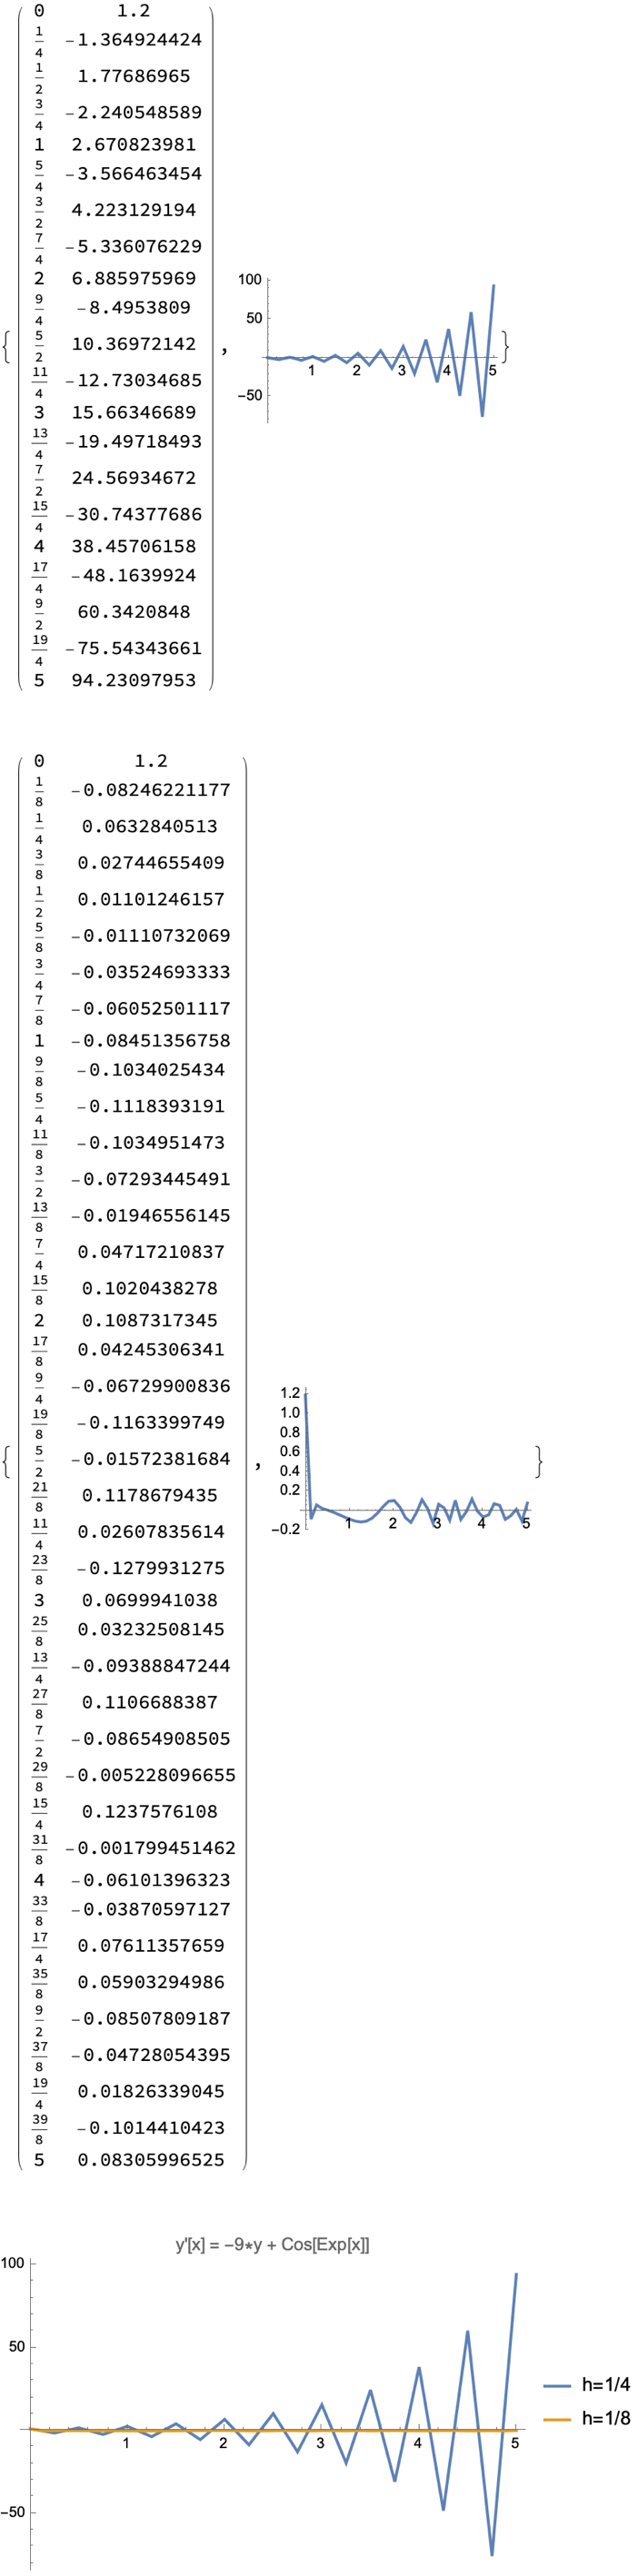
\includegraphics[scale=0.4]{final_q3}
    \end{solution}
    \end{mdframed}
%%%%%%%%%%%%%%%%%%%%%%%%%%%%%%%%%%%%%%%%%%%%%%%%%%%%%%%%%%%%%
    \begin{exercise}
        Single but Exciting Questions!
        \begin{enumerate}[label = (\alph*),itemsep=1pt,topsep=3pt]
            \item Let $T(4n) = 3T(4n-4)$. Determine $T(n)$ explicitly.
            \item Express the number $-219.1963$ as a 64 bit double precision number in IEEE 754 format.
            \item List the eigenvalues and eigenvectors for the matrix:
                \begin{equation*}
                \begin{split}
                    A = \bbmat 3 & 8 & 0 \\ 2 & 3 & 8 \\ 0 & 2 & 3 \ebmat
                \end{split}
                \end{equation*}
            using only an appropriate formula, and without computing the characteristic polynomial or solving any linear systems.
        \end{enumerate}
    \end{exercise}
        \begin{mdframed}
        \begin{solution}
            (a) Let $k  = 4n$. Observe that:
                \begin{equation*}
                \begin{split}
                    T(4n)
                    & = T(k) \\
                    & = 3T(k-4) \\
                    & = 3^2 T(k-8) \\
                    & = 3^3 T(k-16) \\
                    &\vdots
                \end{split}
                \end{equation*} 
            Inductively, $T(k) = 3^\frac{k}{4}T(0)$ for $k \equiv 0 \pmod{4}$. \nl
            
            \noindent (b) The following Mathematica code will express $-219.1963$ as a 64 bit double precision number.
            \begin{mmaCell}[addtoindex=-1,moredefined={Binary, e, f, \
                CellToTeX},morepattern={totalBits_, val_, totalBits, val, \
                cell},morelocal={sbit, ebits,
                mbits, n, j, c, q, r, counter, digit, s, eBits, mBits, bias}]{Input}
Clear["Global`*"]
Binary[totalBits_,val_]:=
  Module[\{sbit=,ebits=,mbits=,n,j,c,q,r,counter,digit,s,
    eBits,mBits,bias\},
   Switch[totalBits,
    16,\{eBits=5;mBits=10;bias=15;\},
    32,\{eBits=8;mBits=23;bias=127;\},
    64,\{eBits=11;mBits=52;bias=1023;\},
    128,\{eBits=15;mBits=112;bias=16383;\},
    256,\{eBits=19;mBits=236;bias=262143;\},
    _,Return[unsupported size]];
  Clear[j,n,c,q,r,counter,digit,s];
  n=Abs[val];
  If[val<0,sbit=1,sbit=0];
  ebits=;
  mbits=;
  If[n<2,e=bias;
    Do[\{q,r\}=QuotientRemainder[e,2];
     ebits=ToString[r]<>ebits;
     e=q;,\{eBits\}];
    f=n-1;
    Do[s=2 f;
     digit=Floor[s];
     mbits=mbits<>ToString[digit];
     f=s-digit;,\{mBits\}];,counter=0;
    While[n>=2,n=n/2;
     counter++;];
    e=counter+bias;
    Do[\{q,r\}=QuotientRemainder[e,2];
     ebits=ToString[r]<>ebits;
     e=q;,\{eBits\}];
    f=n-1;
    Do[s=2 f;
     digit=Floor[s];
     mbits=mbits<>ToString[digit];
     f=s-digit;,\{mBits\}];];
    sbit <>ebits<> mbits]
Binary[64,-219.1963]
\end{mmaCell}
\begin{mmaCell}[addtoindex=2]{Output}
1100000001101011011001100100100000010110111100000000011010001110
\end{mmaCell}

            \phantom{a} \nl
            
            \noindent (c) The eigenvalues of $A$ are given by:
                \begin{equation*}
                \begin{split}
                    \lambda_h(A) = 3 + 4 \cos \left( \frac{h \pi}{4} \right), \h9 h=1,2,3.
                \end{split}
                \end{equation*}
            The corresponding eigenvector of $\lambda_h(A)$ is given by:
                \begin{equation*}
                \begin{split}
                    \bbmat
                        \left( \frac{1}{4} \right)^\frac{1}{2} \sin \left( \frac{h \pi}{4} \right)\\
                        \left( \frac{1}{4} \right) \sin \left( \frac{2h \pi}{4} \right)\\
                        \left( \frac{1}{4} \right)^\frac{3}{2} \sin \left( \frac{3h \pi}{4} \right)\\
                    \ebmat
                \end{split}
                \end{equation*}
        \end{solution}
        \end{mdframed}
%%%%%%%%%%%%%%%%%%%%%%%%%%%%%%%%%%%%%%%%%%%%%%%%%%%%%%%%%%%%%
    \begin{exercise}
        Consider the two equations $x^3 + y^2 = 2$ and $2x^2 + \sin(y) = 3$.
            \begin{enumerate}[label = (\alph*),itemsep=1pt,topsep=3pt]
                \item Research the Mathematica command "ContourPlot". Then plot both of these equations in the same plot on the interval $-3 \leq x,y \leq 3$. Turn in your plot.
                \item If your graph is correct, you should see four points of intersection between the two equations. Using your graph to "suggest" good initial guesses, use an iterative method to determine the four points of intersection $(x_1,y_1),...,(x_4,y_4)$, stable to 4 decimal places.
            \end{enumerate}
    \end{exercise}
        \begin{mdframed}
        \begin{solution}
            (a) The Mathematica cell:
\begin{mmaCell}[addtoindex=3,morefunctionlocal={x, \
y},moredefined={CellToTeX},morepattern={cell}]{Input}
ContourPlot[\{x^3+y^2==2,2 x^2+Sin[y]==3\},\{x,-3,3\},\{y,-3,3\}]
\end{mmaCell}
            outputs the following graph:
                \begin{center}
                    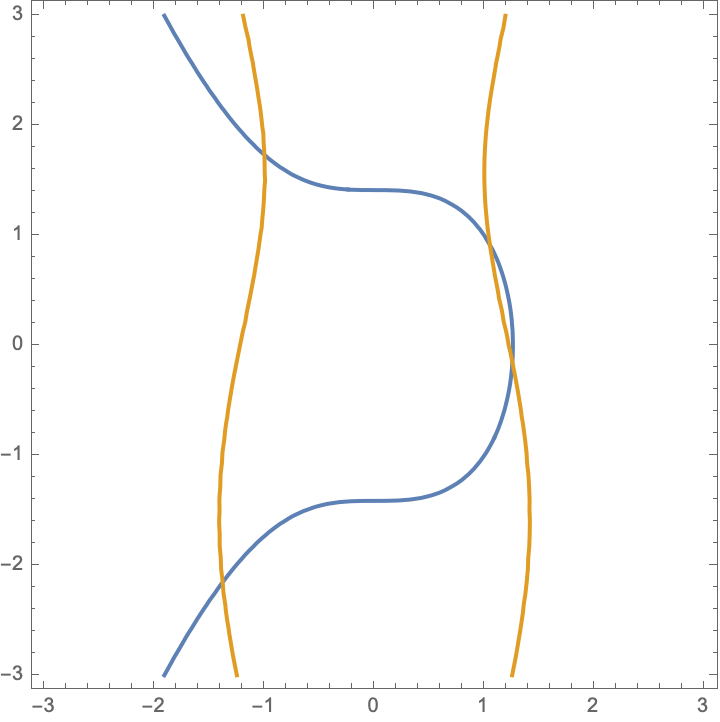
\includegraphics[scale=0.5]{image.png}
                \end{center}
            \phantom{a} \nl
            
            \noindent (b) The following Mathematica code determines all four points of intersection.

\begin{mmaCell}[moredefined={NewtonsMethod, f1, f2, \
table},morepattern={f1_, f2_, x0_, y0_, tol_, maxIter_, maxIter, x_, \
y_, x0, y0, tol},morelocal={xVals,
yVals, delta, n, F, J, sol}]{Input}
Clear["Global`*"]
NewtonsMethod[f1_,f2_,x0_,y0_,tol_:0.0001,maxIter_:20]:=Module[\{
     xVals=ConstantArray[0.,maxIter+1],yVals=ConstantArray[0.,maxIter+1],
     delta,n,F,J,sol\},F[x_,y_]=\{\{f1[x,y]\},\{f2[x,y]\}\};
    J[x_,y_]=\{\{D[f1[x,y],x],D[f1[x,y],y]\},
       \{D[f2[x,y],x],D[f2[x,y],y]\}\};
    xVals[[1]]=N[x0];
    yVals[[1]]=N[y0];
    For[n=1,n<=maxIter,n++,
     delta=Inverse[J[xVals[[n]],yVals[[n]]]].F[xVals[[n]],yVals[[n]]];
     xVals[[n+1]]=xVals[[n]]-delta[[1,1]];
     yVals[[n+1]]=yVals[[n]]-delta[[2,1]];
     If[Max[Abs[\{xVals[[n+1]],yVals[[n+1]]\}-\{xVals[[n]],yVals[[n]]\}]]<tol,
      xVals=Take[xVals,n+1];
      yVals=Take[yVals,n+1];
      Break[]];
    ];
    sol=N[Transpose[\{xVals,yVals\}]];
    table=
     Table[\{\mmaFnc{n}-1,NumberForm[sol[[\mmaFnc{n}]],\{Infinity, 10\},ExponentFunction->(Null&),
           NumberPadding->\{,0\}]\},\{\mmaFnc{n},Length@sol\}];
    TableForm[Prepend[table,\{n,"(x,y)"\}]]]

f1[x_,y_]=x^3+y^2-2;
f2[x_,y_]=2 x^2+Sin[y]-3;
NewtonsMethod[f1,f2,1,1]
NewtonsMethod[f1,f2,-1,-2]
NewtonsMethod[f1,f2,-1,2]
NewtonsMethod[f1,f2,1,-1]
\end{mmaCell}

\newpage
\begin{mmaCell}[addtoindex=-267,form=TableForm]{Output}
n	(x,y)
0	\{1.0000000000,1.0000000000\}
1	\{1.0497026813,0.9254459781\}
2	\{1.0502192250,0.9174500191\}
3	\{1.0502341737,0.9173877601\}
\end{mmaCell}

\begin{mmaCell}[form=TableForm]{Output}
n	(x,y)
0	\{-1.0000000000,-2.0000000000\}
1	\{-1.4669022999,-2.1001767249\}
2	\{-1.3871062327,-2.1550829268\}
3	\{-1.3843773549,-2.1571122515\}
4	\{-1.3843741591,-2.1571142160\}
\end{mmaCell}

\begin{mmaCell}[form=TableForm]{Output}
n	(x,y)
0	\{-1.0000000000,2.0000000000\}
1	\{-0.9963843454,1.7472882591\}
2	\{-1.0033616158,1.7349710779\}
3	\{-1.0033556981,1.7349642401\}
\end{mmaCell}

\begin{mmaCell}[form=TableForm]{Output}
n	(x,y)
0	\{1.0000000000,-1.0000000000\}
1	\{1.3828061119,-0.4257908322\}
2	\{1.2718843155,-0.2036910745\}
3	\{1.2557034631,-0.1534251740\}
4	\{1.2551061728,-0.1511568631\}
5	\{1.2551050824,-0.1511524435\}
\end{mmaCell}
        \end{solution}
        \end{mdframed}
%%%%%%%%%%%%%%%%%%%%%%%%%%%%%%%%%%%%%%%%%%%%%%%%%%%%%%%%%%%%%
\end{document}